\chapter{Safety and Security}
\label{chap:safety_and_security}

\acp{iommu} have been bypassed in numerous ways due to weaknesses in \ac{pcie},
boot-time issues and poor configuration of \acp{iommu} by \acp{os}. We describe
some attacks to give a short overview of vulnerabilities. In the second half of
the chapter (\Cref{sec:iotlb}), we take a closer look at the \ac{iotlb} of
\acp{iommu} which we assume to be another weak point. We suspect that the
\ac{iotlb} is susceptible to timing attacks.


\section{Known Vulnerabilities}
\label{sec:known_vulnerabilities}

On the \ac{pcie} level, two flaws stand out. First, devices can impersonate
other \ac{pcie} devices by spoofing their \ac{pcie} ID (i.e., the \ac{bdf}).
Since \acp{iommu} perform address translation and check access permissions based
on the \ac{pcie} ID of \ac{pcie} packets, devices can access memory assigned to
other devices by spoofing their ID. When \acp{iommu} are used in pass-through
mode, i.e., only some devices use the \ac{iommu}, devices may even bypass the
\ac{iommu} completely and access all memory of a host. Access in this context
refers primarily to write access. For read access, routing configuration has to
be updated. This is theoretically possible but rather unlikely in practice.
Daubignard and Perez explain the attack vector in more detail
\cite{daubignard2017protip}.

Second, devices may implement a \ac{pcie} capability called Address Translation
Services (ATS). With ATS, devices announce that they are capable of caching
address translations and translate addresses of \ac{dma} requests on their own.
Thus, ATS reduces pressure on the \ac{iotlb} of \acp{iommu}. Devices using this
capability request translations from \ac{dma} remapping hardware, cache the
translations and receive invalidation requests once address mappings are no
longer valid. \ac{pcie} memory read and write requests of such devices indicate
whether the specified address was translated by the device or still needs to be
translated (by the \ac{iommu}). If ATS is enabled for a device, memory requests
with translated addresses pass the remapping hardware unchecked. There are no
restrictions on which addresses can be accessed by a device, malicious or faulty
devices can masquerade any address as legitimately translated address.

Both flaws in the \ac{pcie} protocol can be mitigated (to a certain point) using
a \ac{pcie} feature named Access Control Services (ACS). With ACS, ports of the
root complex and switches can be configured to verify whether the \ac{pcie} ID
used in a request belongs to a port's subset of bus numbers. Furthermore, memory
requests with ATS-translated addresses can be blocked. These operations are
known as source validation and translation blocking. However, ACS is an optional
\ac{pcie} feature and might not or only partially be available on a system
\cite[p.~582]{pcie2017specification}.

In case ACS is not available, ATS can still be disabled in the \ac{iommu}. Both
Intel's and AMD's \acp{iommu} check memory requests with translated addresses
for eligibility, i.e., whether ATS is enabled. Intel stores this information in
the context entry of the domain, AMD in the device entry.

Other attack vectors exist at boot-time: On some architectures, \acp{iommu}
could be hidden from the \ac{os} by rewriting the \ac{dmar} \ac{acpi} tables at
boot-time \cite{wojtczuk2009another}. Morgen et al. used another weakness and
rewrote the tables of the \ac{iommu} during initialization, setting the
translation type of \ac{iommu} domains to pass-through mode
\cite{morgan2018iommu}.

The flaws in how \aclp{os} configure \acp{iommu} are even worse. In 2019,
Markettos et al. examined the behavior of all major \acp{os} and came to
disillusioning conclusions \cite{markettos2019thunderclap}. Most versions of
Microsoft Windows did not use the \ac{iommu} at all and were therefore entirely
unprotected against \ac{dma} attacks. Windows 10 Enterprise supported
\acp{iommu}, however, they were only used to protect a secure container (VBS),
not the root operating system. Unlike Windows, macOS and Linux enabled
\acp{iommu}. However, \ac{dma} memory was shared between devices on macOS and
both \aclp{os} exposed \ac{os} data structures to the devices. Markettos et al.
show 5 different ways on macOS and Linux to bypass the \ac{iommu}, some so
serious that a root shell could be obtained.

Following the revelations of Markettos et al., \ac{os} vendors released
mitigations against the newly discovered vulnerabilities. Besides, Microsoft
announced to support \acp{iommu} as of Windows 10 version 1803, and Linux
disabled ATS entirely for external devices (e.g., Thunderbolt). However,
internal hardware is still considered trustworthy. To reduce the surface area
for attacks sustainably, Markettos et al. call for a fundamental change of the
thread models of operating systems and drivers.


\section{The IOTLB}
\label{sec:iotlb}

We suspect that there exists yet another vulnerability in \acp{iommu} in
relation to \acp{iotlb}, which are used by \acp{iommu} to cache information
about domains and address mappings to accelerate address lookup. To be more
precise, we suspect that these \acp{iotlb} -- just like other caches -- are
vulnerable to timing attacks, i.e., multiple devices or functions share the same
\ac{iotlb} and \ac{dma} access times depend on availability of translation
information in the cache.

We implement an application on top of the methods described in
\Cref{sec:iommu_leaks} to run some timing measurements on \ac{dma} operations.
Our application follows the idea of priming and probing: By carefully
controlling the \ac{dma} accesses of the \ac{nic}, we try to bring the
\ac{iotlb} into a known state. We run our measurements on the Intel Xeon E5
\ac{cpu} as it is the only \ac{cpu} that supports \ac{sriov} with \ac{iommu} and
two devices.

We assume that the \ac{iotlb} of this \ac{cpu} has 64 entries. We allocate 64
physically and virtually contiguous 4~KiB pages, place the TX descriptor ring on
the first page and use the other 63 pages for our packets. We use one port of
the Intel X520-DA2 \ac{nic} for our application and configure the device to use
our 64 pages. We disable the RX queue of the device to prevent \ac{dma} accesses
on packet arrival.

\begin{figure}%[!b]
    \centering
    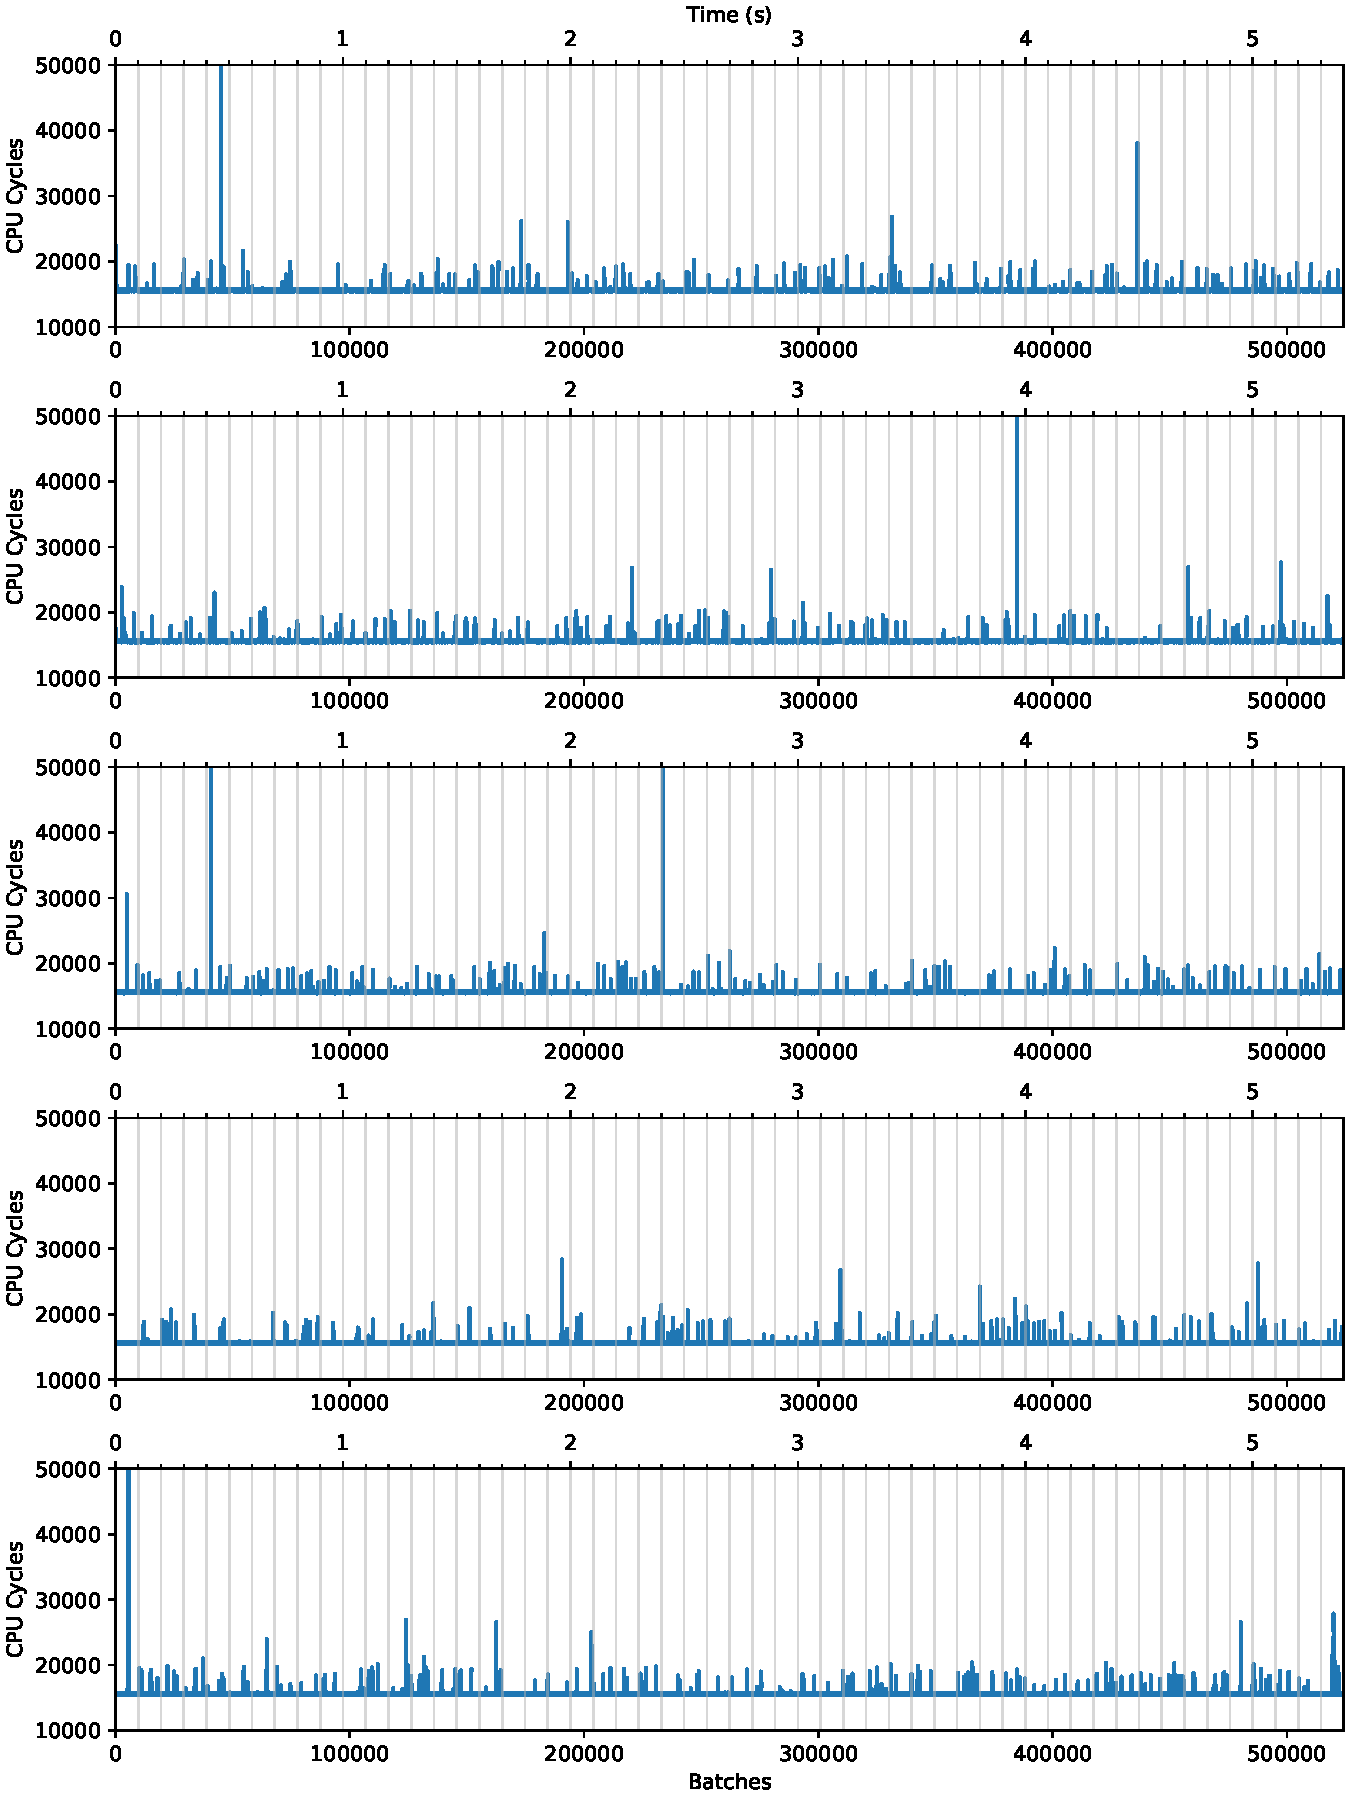
\includegraphics[width=1.0\textwidth]{figures/iotlb-baseline-no-iommu}
    \caption{CPU cycles per batch of transmitted packets.}
    \label{fig:cycles-no-iommu}
\end{figure}

\begin{figure}%[!b]
    \centering
    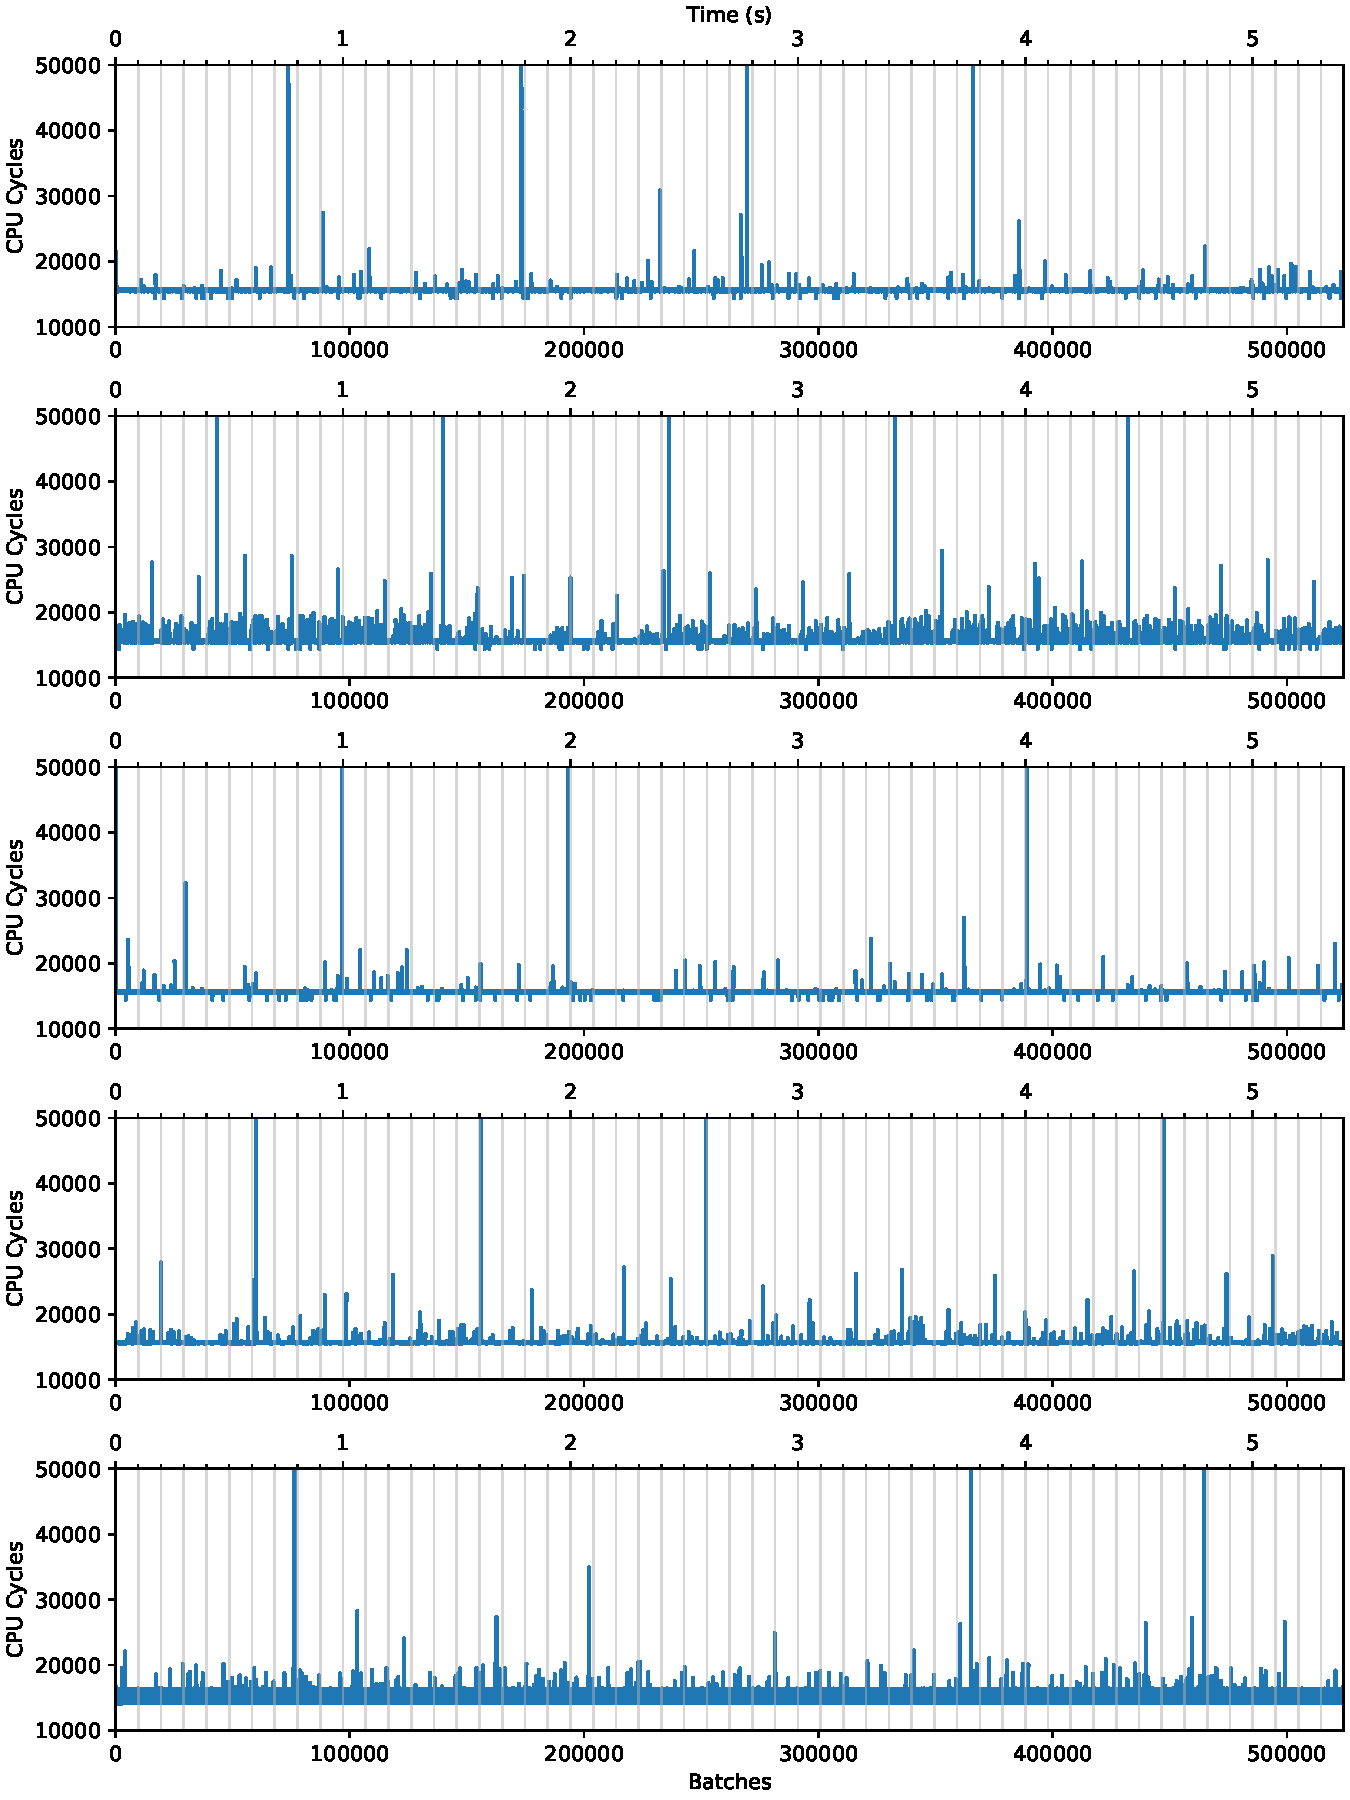
\includegraphics[width=1.0\textwidth]{figures/iotlb-baseline-iommu-pt}
    \caption{CPU cycles per batch of transmitted packets with IOMMU.}
    \label{fig:cycles-iommu-pt}
\end{figure}

\begin{figure}%[!b]
    \centering
    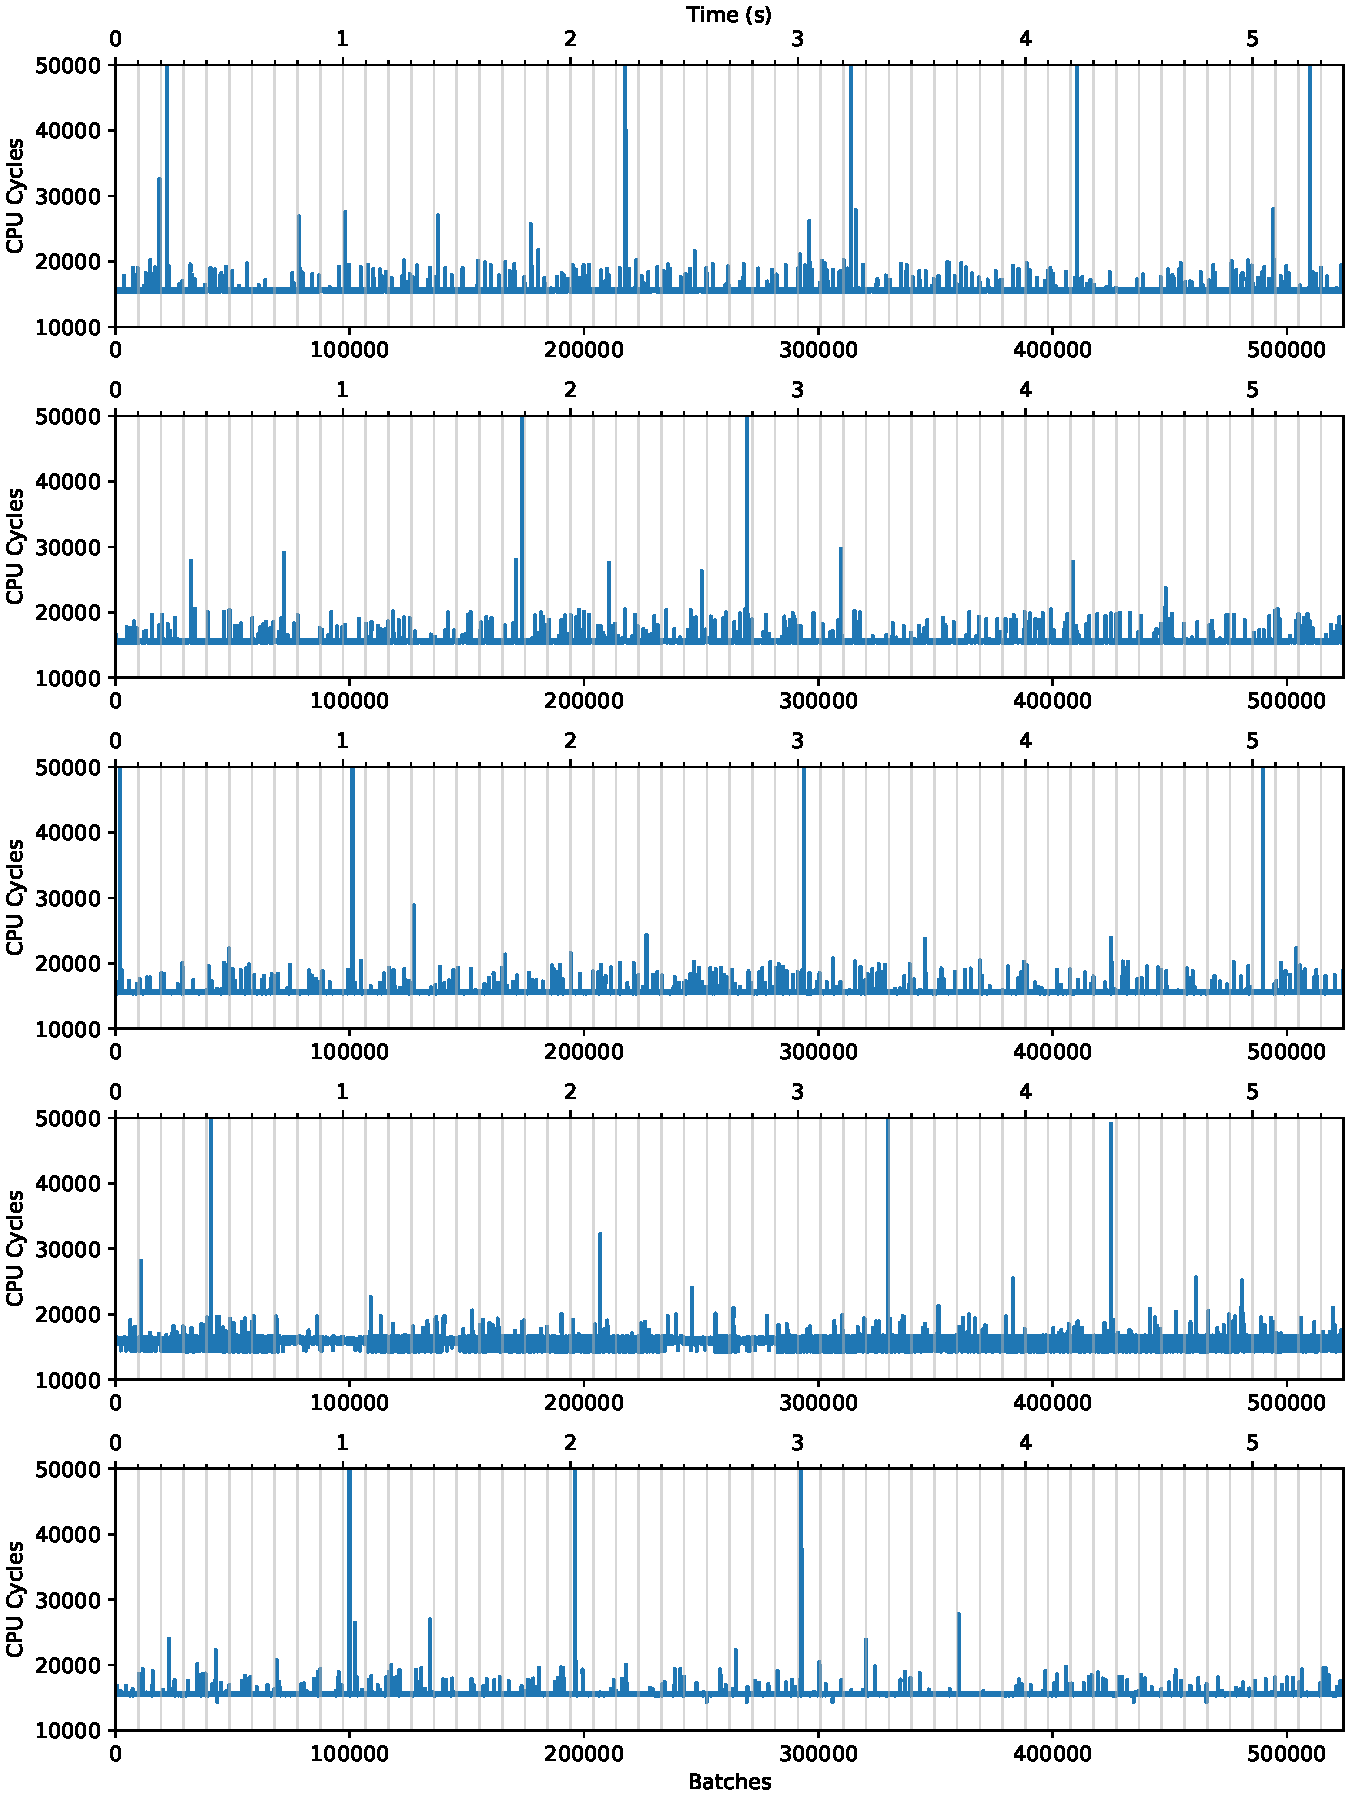
\includegraphics[width=1.0\textwidth]{figures/iotlb-baseline-iommu-pt-fixed}
    \caption{CPU cycles per batch of transmitted packets with IOMMU and fixed
    virtual and physical addresses.}
    \label{fig:cycles-iommu-pt-fixed}
\end{figure}

\begin{figure}%[!b]
    \centering
    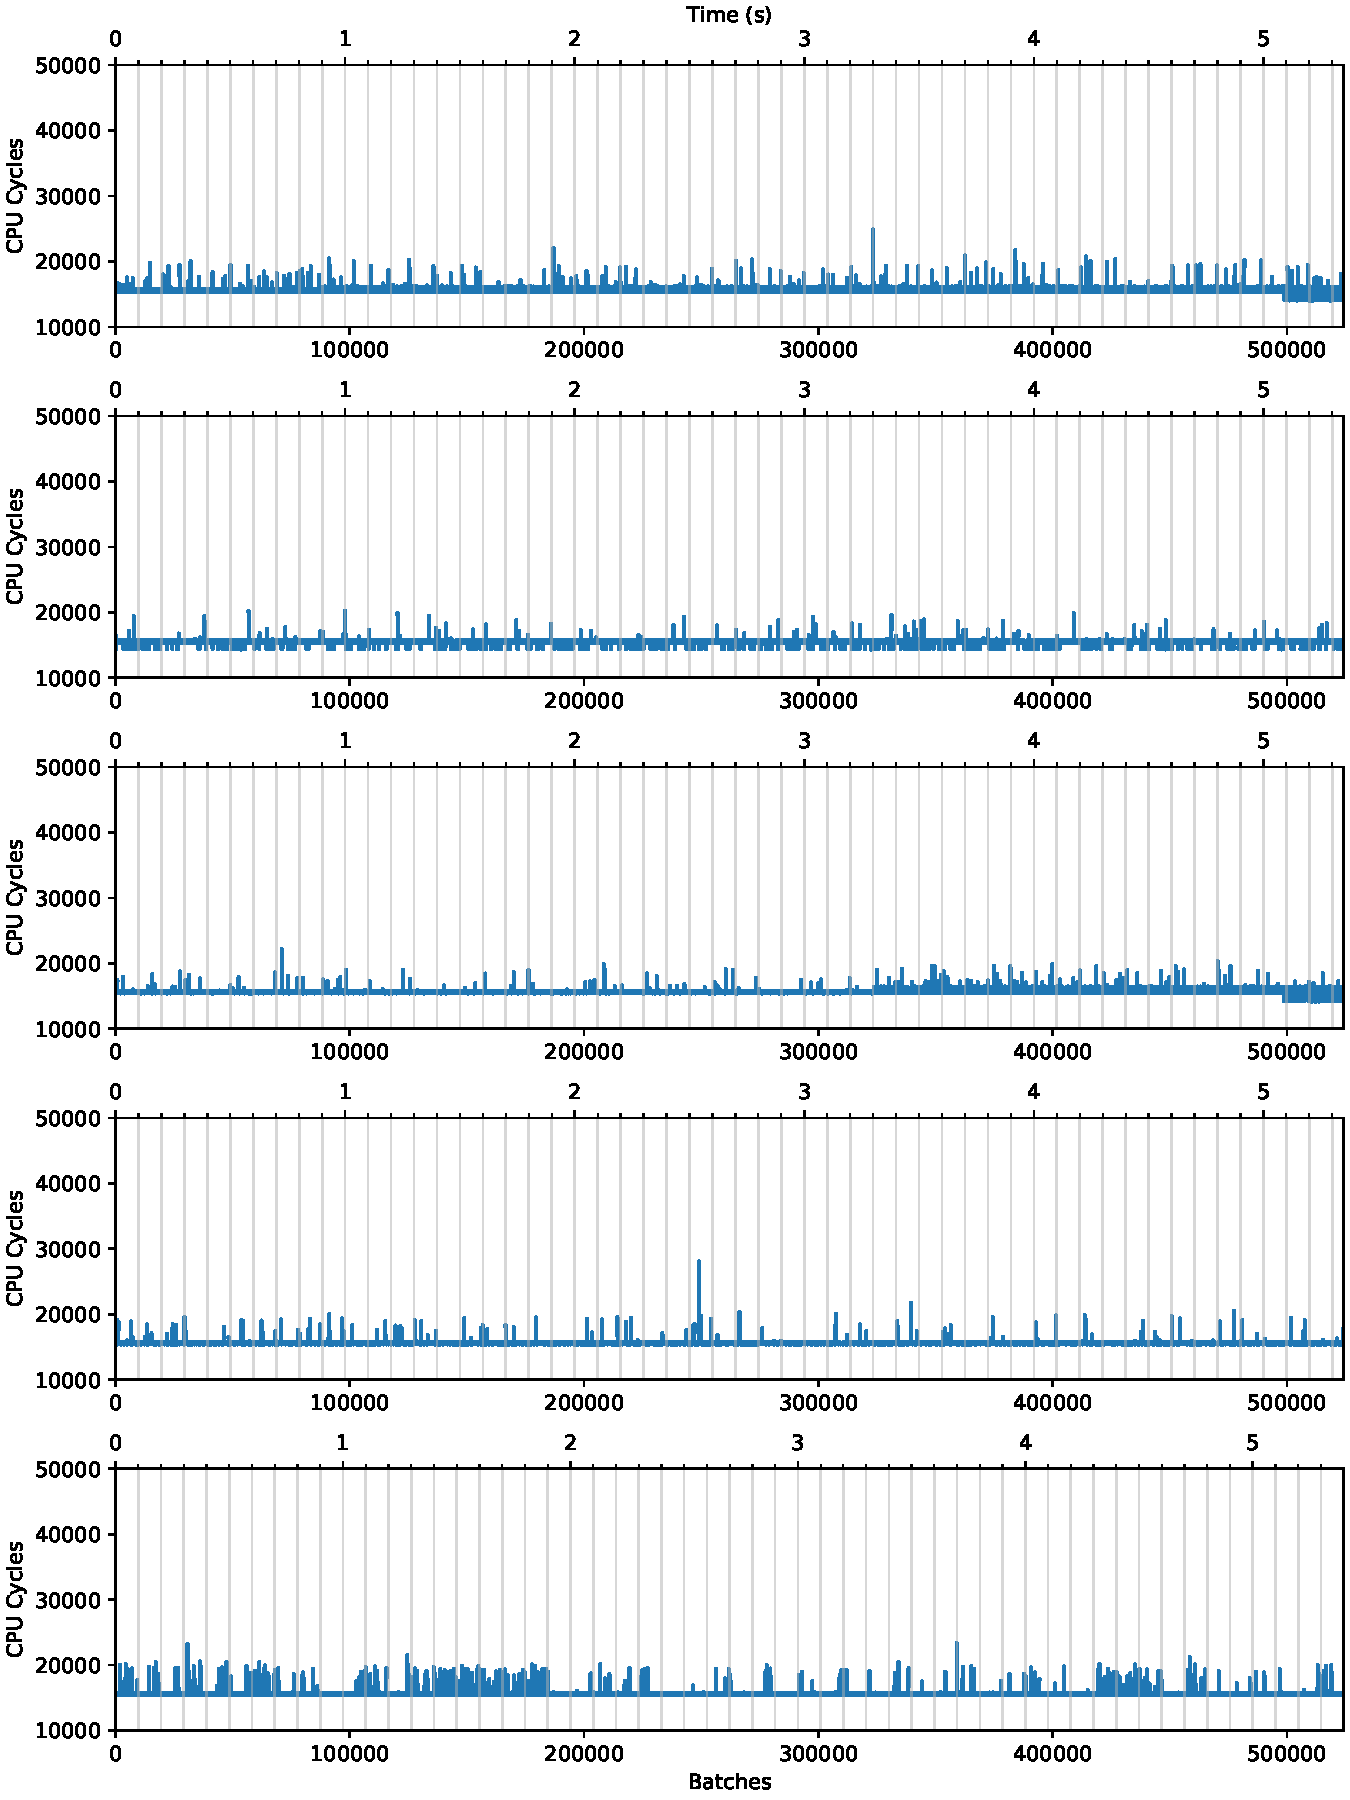
\includegraphics[width=1.0\textwidth]{figures/iotlb-baseline-iommu-pt-fixed-no-devs}
    \caption{CPU cycles per batch of transmitted packets with IOMMU and fixed
    virtual and physical addresses, other PCIe devices unbound.}
    \label{fig:cycles-iommu-pt-fixed-no-devs}
\end{figure}

\begin{figure}%[!b]
    \centering
    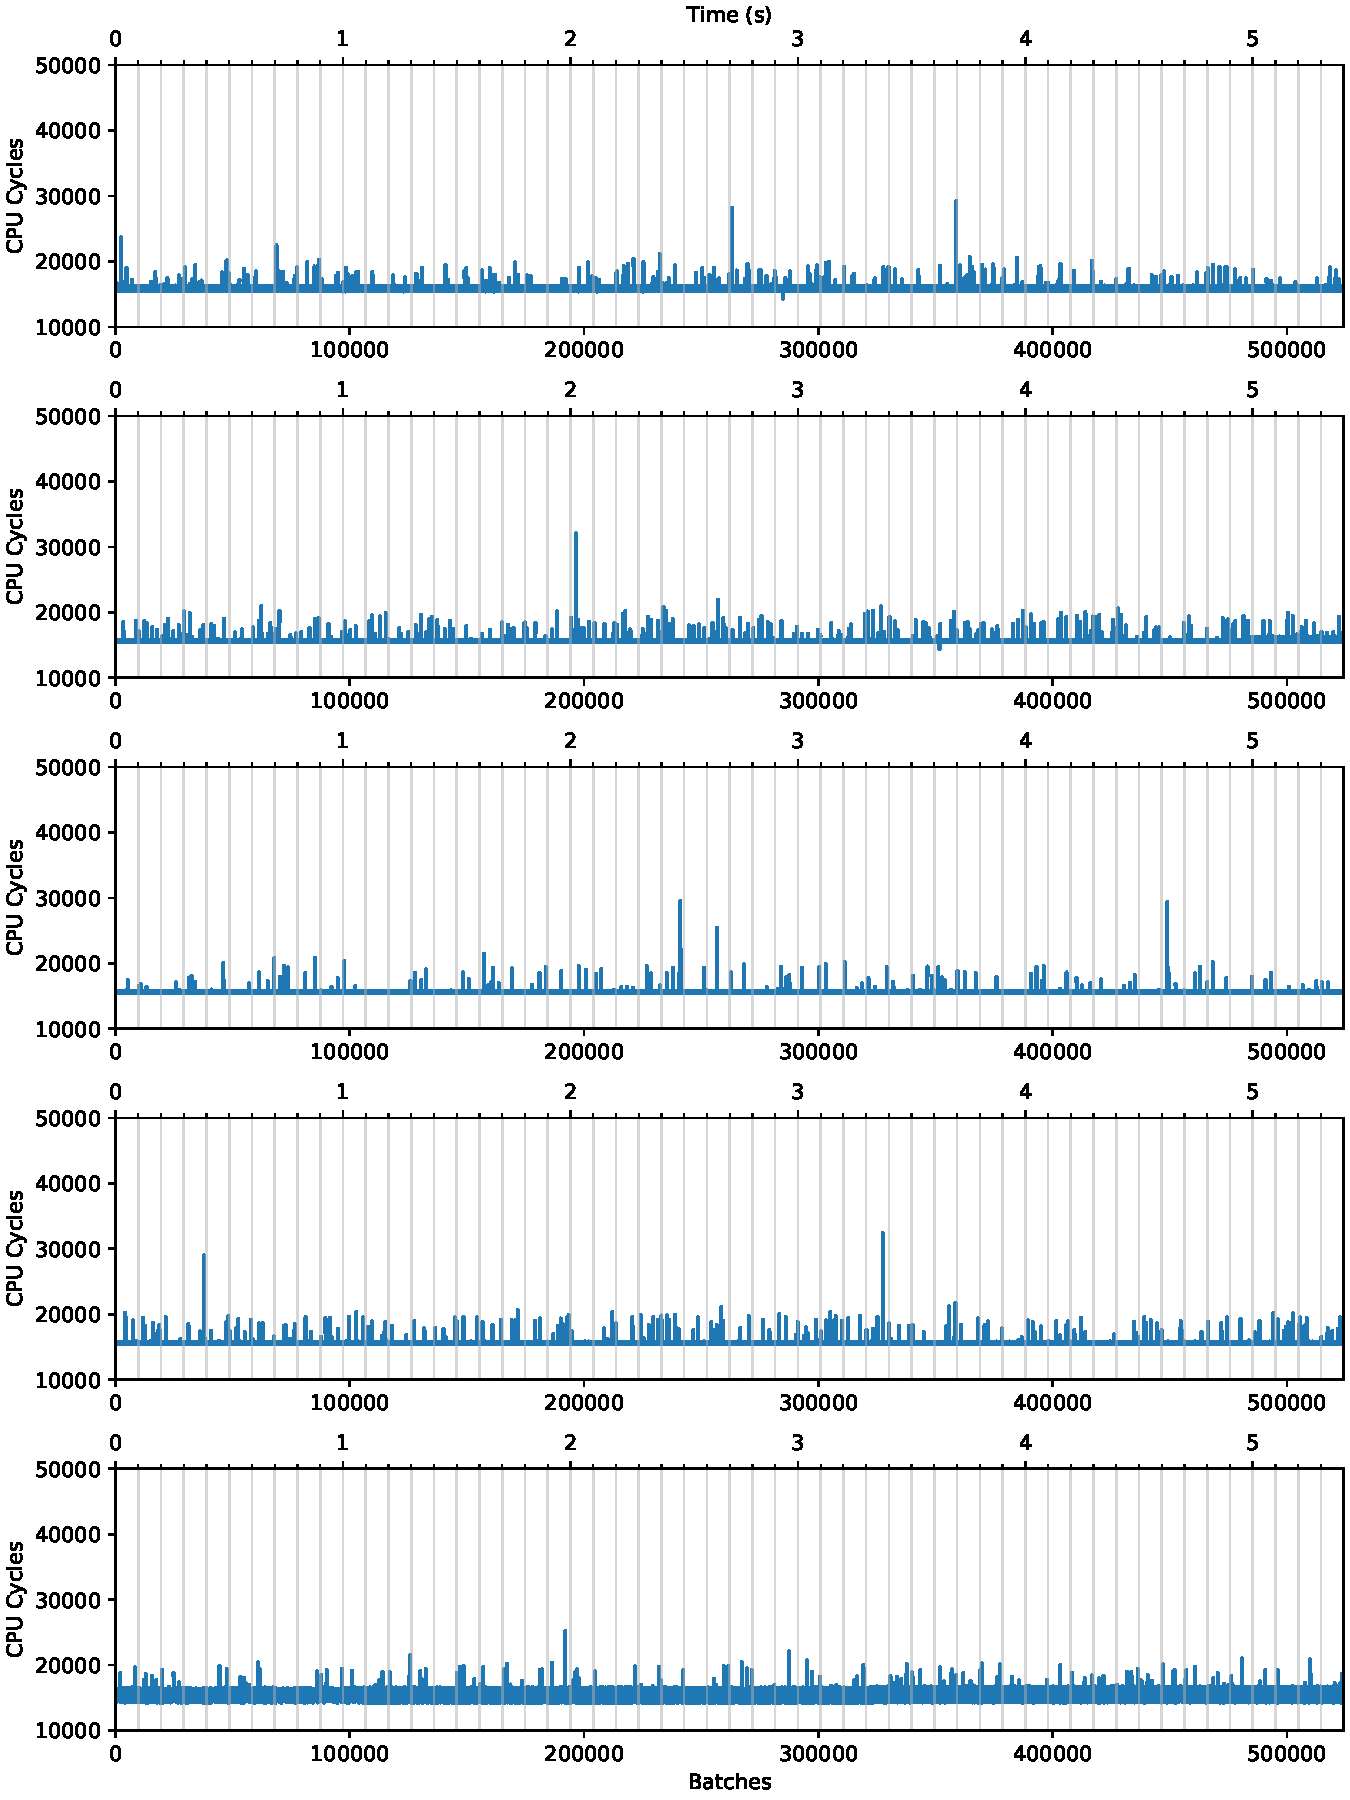
\includegraphics[width=1.0\textwidth]{figures/iotlb-baseline-iommu-pt-fixed-no-devs-ping-0.4}
    \caption{CPU cycles per batch of transmitted packets with IOMMU and fixed
    virtual and physical addresses, other PCIe devices unbound, ping on second
    NIC port every 0.4 seconds.}
    \label{fig:cycles-iommu-pt-fixed-no-devs-ping}
\end{figure}

In our first measurements, we try to determine the number of \ac{cpu} cycles it
takes for the \ac{nic} to fetch the TX descriptors from one page, transmit a
batch of 63~packets from the 63~other pages, and set the descriptor-done bit in
the last TX descriptor on the descriptor page. Thus, the \ac{nic} accesses
64~distinct but physically and virtually contiguous pages for every batch of
to-be-transmitted packets.

We run the application with and without \ac{iommu}. We warm up the caches before
starting our measurements. For every run of the application, we measure the
\ac{cpu} cycles for 500k batches and mean and standard deviation of the
\ac{cpu} cycles. \Cref{fig:cycles-no-iommu} shows the results of five runs
without \ac{iommu}. The plots are cut off at 50,000~\ac{cpu} cycles, all spikes
that end up at 50,000~cycles go up to 400,000~\ac{cpu} cycles.

Several conclusions can be drawn from the plots. First, the number of \ac{cpu}
cycles varies greatly in every run. Second, the number of \ac{cpu} cycles
between spikes is constant in a run and for all runs. Third, some spikes appear
equidistantly across runs, e.g., with a time interval of 0.4, 0.6 or
\SI{2.0}{\s}.

On average, we note 15,622~\ac{cpu} cycles and a standard deviation of
623~cycles for the runs in \Cref{fig:cycles-no-iommu}. With a batch size of
63~packets, we get 248~cycles per packet.

We repeat our measurements with the \ac{iommu} in pass-through mode, i.e.,
our device uses the \ac{iommu}. \Cref{fig:cycles-iommu-pt} shows the results.
Notably, variance of the \ac{cpu} cycles is even worse with \ac{iommu}. However,
we can also notice more patterns in the spikes. In the second run from the top,
spikes between 22k and 30k~\ac{cpu} cycles appear every \SI{0.2}{\s}, and spikes
above 50,000~\ac{cpu} cycles every second.

On average, we note 15,682~\ac{cpu} cycles and a standard deviation of
658~cycles for the runs in \Cref{fig:cycles-iommu-pt}. With a batch size of
63~packets, we get 249~cycles per packet. Thus, we put the cost of the
\ac{iommu} at 60~cycles per batch of packets or about 1~cycle per packet.

To minimize variance between runs, we modify our application such that the same
virtual and physical memory addresses are used for every run. We allocate a
chunk of physical memory on boot using the Linux kernel's \texttt{memmap} flag
and \texttt{mmap} the memory chunk into the process address space via
\texttt{/dev/mem}.

\Cref{fig:cycles-iommu-pt-fixed} shows the results of running our application
with \ac{iommu} and fixed addresses. To our disappointment, \ac{cpu} cycles
still vary greatly although all runs were executed on the same \ac{cpu} core
with the same memory addresses and no dynamic overclocking. Again, we note a
periodicity of the peaks of 1.0 and \SI{2.0}{\s}.

As a final attempt, we unbind all \ac{pcie} devices not needed for our
measurements and repeat our measurements with fixed memory addresses.
\Cref{fig:cycles-iommu-pt-fixed-no-devs} shows that without these \ac{pcie}
devices, background noise is reduced significantly. However, our measurements
still contain too much variance to draw conclusions about \ac{iotlb} misses. We
verify this assumption by binding the second part of the \ac{nic} to the kernel
\texttt{ixgbe} driver and sending out ping packets every \SI{0.4}{\s}.
\Cref{fig:cycles-iommu-pt-fixed-no-devs-ping} depicts the results of the same
measurements with ping running on the second port of the \ac{nic}. The plots
confirm our assumption. We cannot determine the ping packets with our
measurements.


\section{Summary}
\label{sec:sec_summary}

\acp{iommu} provide limited protection against malicious or faulty peripherals
due to weaknesses in the \ac{pcie} protocol. Besides, architectural flaws,
missing support and incorrect handling of \acp{iommu} by \aclp{os} further
reduce the safety / security benefits of employing \acp{iommu}.

Although we suspect the possiblity of side-channel attacks using the \ac{iotlb},
our timing measurements in \Cref{sec:iotlb} do not reveal any significant
differences between non-\ac{iommu} and \ac{iommu} usage. Our measurements prove
to have far too much variance to detect any individual \ac{iotlb} misses.

